
% TODO: https://en.wikipedia.org/wiki/Triangle

\index{pons asinorum|(}
\section{Pons asinorum}
%

,,\emph{Pons asinorum}'', czyli most osłów, to tradycyjna nazwa twierdzenia (I.5), że kąty przy podstawie trójkąta równoramiennego są równe.
Ci, którzy nie są w stanie samodzielnie przeprowadzić jego dedukcyjnego dowodu opartego na własnościach trójkątów przystających, nie mogą przekroczyć mostu i studiować dalej geometrii.
Bardziej przyziemnie Coxeter \cite[s. 22-24]{coxeter_1967} zauważa, że rysunek wykonany przez Euklidesa przypomni most.
Wśród konsekwencji wymienia wyniki z~Elementów: (III.3), (III.20), (III.21), (III.22), (III.32), (VI.2), (VI.4), a potem (III.35), (III.36), (VI.19), co prowadzi do dowodu twierdzenia Pitagorasa, czyli (I.47). % TODO: sprawdzić, czy numeracja moja i Coxetera jest taka sama.
\index{twierdzenie!Pitagorasa}%

\begin{figure}[H] \centering
\begin{comment}
\begin{tikzpicture}[scale=.5]
    \tkzDefPoint(90:-1){A}
    \tkzDefPoint(-55:5){C}
    \tkzDefPoint(235:5){B}
    \tkzDefPoint(-90:8){X}

    \tkzLabelPoint[above](A){$A$}
    \tkzLabelPoint[left](B){$B$}
    \tkzLabelPoint[right](C){$C$}
    \tkzInterLC(A,B)(A,X) \tkzGetPoints{XX}{D} % line and circle
    \tkzLabelPoint[left](D){$D$}
    \tkzDefLine[parallel=through D](B,C) \tkzGetPoint{XXX}
    \tkzInterLL(D,XXX)(A,C) \tkzGetPoint{E} % line and circle
    \tkzLabelPoint[right](E){$E$}
    
    \tkzMarkSegments[mark=|](A,B A,C)
    \tkzMarkSegments[mark=||](B,D C,E)
    \tkzDrawLines[add= 0 and 0, line width=0.2mm](B,E C,D)
    \tkzDrawLines[add= 0 and 0.5, line width=0.2mm](B,D C,E)
    \tkzDrawPolygon[line width=0.5mm](A,B,C)
    \tkzDrawPoints[size=4,color=black,fill=black!50](A,B,C,D,E)
\end{tikzpicture}
\end{comment}
    \caption{most osłów}
\end{figure}

Pierwsze dowody tego faktu podadzą jeszcze Euklides, komentujący jego prace Proklos, a także (dużo krócej\footnote{Pappus zauważa, że trójkąt $\triangle ABC$ przystaje do siebie $\triangle ACB$, więc stosowne kąty przy podstawie też są przystajace.}) Pappus z Aleksandrii.
\index[persons]{Proklos zwany Diadochem}%
\index[persons]{Pappus z Aleksandrii}%
Przyszłość przyniesie jeszcze jedno uzasadnienie, zaczynające się od wykreślenia dwusiecznej z kąta przy wierzchołku.
\index{dwusieczna}%
Euklides nie zrobi tego przede wszystkim ze względu na kolejność wykładanego materiału: dwusieczna pojawi się cztery tezy później, a nie można korzystać z wyników, których prawdziwości dopiero się pokaże.

O pons asinorum nie wspomina żaden szkolny podręcznik geometrii \texttt{:(}
Pojawia się u Bogdańskiej, Neugebauera \cite[s. 9]{neugebauer_2018}.

% PRZECZYTANO: https://en.wikipedia.org/wiki/Pons_asinorum

%
\index{pons asinorum|)}
\index{most osłów|see{pons asinorum}}

\section{Nierówność trójkąta}
%

Zajmiemy się teraz (I.20).

\begin{proposition}[nierówność trójkąta]
\index{nierówność!trójkąta}%
	Niech $ABC$ będzie trojkątem.
	Wtedy suma odcinków $AB$ i $BC$ jest dłuższa niż $AC$.
\end{proposition}
% PRZECZYTANO: https://en.wikipedia.org/wiki/Triangle_inequality

\begin{proof}
	Wynika to ze wzoru Herona (fakt \ref{prp_heron}) i tego, że pole trójkąta jest nieujemne.
\end{proof}

\begin{corollary}
	Niech $a \ge b \ge c$ będą bokami trójkąta.
	Wtedy
	% \begin{equation}
	% 	1 < \frac{a + c}{b} < 3 
	% \end{equation}
	% oraz
	\begin{equation}
		1 \le \min \left(\frac ab, \frac bc\right) \le \phi = \frac {1 + \sqrt 5}{2}.
		% American Mathematical Monthly, pp. 49-50, 1954. 
	\end{equation}
\end{corollary}

Nierówność trójkąta nie jest wnioskiem z aksjomatów I1-I3, B1-B4, C1-C3, ponieważ nie zachodzi w następującym modelu (ukradniętym Hartshorne'owi \cite[s. 90]{hartshorne2000}):

\begin{example}
	Rozpatrujemy zbiór $\mathbb R^2$ jako płaszczyznę ze standardowymi punktami oraz prostymi, ale niestandardową metryką
	\begin{equation}
		d((x_1, y_1), (x_2, y_2)) = \begin{cases}
			\sqrt{(x_1-x_2)^2 + (y_1-y_2)^2} & \text{jeśli } x_1 = x_2 \vee y_1 = y_2, \\
			2 \sqrt{(x_1-x_2)^2 + (y_1-y_2)^2} & \text{w przeciwnym wypadku}
		\end{cases}.
	\end{equation}
	Wtedy nierówność trójkąta nie zachodzi.
\end{example}

% section{Problemy Fagnano i Fermata}
% https://en.wikipedia.org/wiki/Fagnano's_problem

\begin{problem}[zadanie Fagnano]
	Dany jest trójkąt ostrokątny $ABC$.
	Wpisać w niego trójkąt $UVW$ o możliwie najmniejszym obwodzie.
\index{zadanie!Fermata}%
\end{problem}

Coxeter \cite[s. 36, 37]{coxeter_1967} pokaże tak jak Fejer, że rozwiązaniem zadania jest trójkąt spodkowy (zwany ortycznym).
Audin \cite[s. 101]{audin_2003} podaje ten fakt w formie ćwiczenia. % todo: fagnano czy gemrat?

\begin{problem}[zadanie Fermata]
	\label{punkt_fermata}
	Dany jest trójkąt ostrokątny $ABC$.
	Znaleźć punkt $F$ taki, by suma $|FA| + |FB| + |FC|$ była możliwie najmniejsza.
\index{zadanie!Fermata}%
\end{problem}

\todofoot{Zadanie Fermata -- Neugebauer, s. 117.}

Powyższe zadanie rozwiąże Evangelista Torricelli (dlatego też punkt $F$ nazywa się czasem punktem Torricellego; robi tak Guzicki \cite[s. 224-228]{guzicki_2021}), który dostanie je w formie wyzwania od Fermata.
\index[persons]{Torricelli, Evangelista}%.
Rozwiązanie opublikuje student Torricelliego, Vincenzo Viviani, w 1659 roku.
\index[persons]{Viviani, Vincenzo}
% TODO: Johnson, R. A. Modern Geometry: An Elementary Treatise on the Geometry of the Triangle and the Circle. Boston, MA: Houghton Mifflin, pp. 221-222, 1929.
Coxeter \cite[s. 37]{coxeter_1967} przytoczy rozwiązanie Hofmanna\todofoot{J E Hoffman, Elementare Losung einer Mimimumsaufgabe 1929}
\index{zadanie!Fagnano}

%

\section{Punkty szczególne}
Z każdym trójkątem związane są pewne specjalne punkty, internetowa lista \emph{Encyclopedia of Triangle Centers} wymieni ich co najmniej 68 547.
My nie mamy aż tyle miejsca, więc ograniczymy się do najważniejszych.

$X(1)$ to środek okręgu wpisanego, 
$X(2)$ to środek ciężkości,
$X(3)$ to środek okręgu opisanego,
$X(4)$ to ortocentrum.
Te cztery punkty opisujemy poniżej.

$X(5)$ to środek okręgu dziewięciu punktów z faktu \ref{okrag_dziewieciu_punktow},
$X(6)$ to punkt Lemoine'a (Grebego) z faktu \ref{punkt_lemoine},
$X(7)$ to punkt Gergonne'a z~faktu \ref{punkt_gergonne},
$X(8)$ to punkt Nagela z faktu \ref{punkt_nagela}, 
$X(9)$ to mittenpunkt (punkt Lemoine'a trójkąta rozpiętego przez środki okręgów dopisanych; leży na prostych łączących środek ciężkości z punktem Gergonne'a, środek okręgu wpisanego z punktem Lemoine'a oraz ortocentrum ze środkiem Spiekera), % https://en.wikipedia.org/wiki/Mittenpunkt
$X(10)$ to środek okręgu Spiekera z faktu \ref{punkt_spiekera},
$X(11)$ to punkt Feuerbacha z twierdzenia \ref{punkt_feuerbacha},
$X(13)$ to punkt Fermata z zadania \ref{punkt_fermata},
$X(17)$, $X(18)$ to punkty Napoleona,
$X(39)$ to środek odcinka łączącego punkty Brocarda z definicji \ref{punkty_brocarda}.
Lista jest długa, a jej końca nie widać.

\subsubsection{Trzy symetralne}
\begin{proposition}
    \label{symetralne_przecinaja_sie}
    Trzy symetralne boków trójkąta przecinają się w jednym punkcie, środku okręgu opisanego na tym trójkącie.
\end{proposition}

Wynika to bezpośrednio z uwagi za definicją \ref{def_symetralna}: w trójkącie $\triangle ABC$, symetralna boku $AB$ (odpowiednio: $AC$) zawiera środki okręgów przechodzących przez punkty $A$ oraz $B$ (przez punkty $A$ oraz $C$), zatem trzecia symetralna musi przejść przez punkt wspólny dwóch pierwszych.

Hartshorne \cite[s. 16]{hartshorne2000} podaje to w formie ćwiczenia ze wskazówką, by spojrzeć na (IV.5).
Audin \cite[s. 61]{audin_2003} też, ale bez wskazówki.
Inne odsyłacze to Neugebauer \cite[s. 19]{neugebauer_2018}.

\begin{proposition}
	Środek okręgu opisanego na trójkącie leży wewnątrz tego trójkąta (odpowiednio: na jego brzegu, na zewnątrz trójkąta) wtedy i tylko wtedy, gdy trójkąt jest ostrokątny (odpowiednio: prostokątny, rozwartokątny).
\end{proposition}

Uogólnieniem faktu \ref{symetralne_przecinaja_sie} o współpękowości symetralnych boków trójkąta jest:

\begin{theorem}[Carnota]
\index{twierdzenie!Carnota}%
\label{guzicki_6_13}%
	Dany jest trójkąt $ABC$ i punkty $D, E, F$ leżące odpowiednio na prostych $BC, CA, AB$.
	Niech prosta $k$ (odpowiednio: $l$, $m$) przechodzi przez punkt $D$ ($E$, $F$) i będzie prostopadła do prostej $BC$ ($CA$, $AB$).
	Wtedy proste $k$, $l$, $m$ mają punkt wspólny wtedy i tylko wtedy, gdy
	\begin{equation}
		|AF|^2 + |BD|^2 + |CE|^2 = |AE|^2 + |BF|^2 + |CD|^2.
	\end{equation}
\end{theorem}
% TODO: https://en.wikipedia.org/wiki/Carnot%27s_theorem_(perpendiculars)

Guzicki \cite[s. 176]{guzicki_2021} wyprowadza je z twierdzenia Pitagorasa, co pozwala mu dojść do wniosku, że okręgi opisany i wpisany oraz ortocentrum istnieją.
\index{twierdzenie!Pitagorasa}

\subsubsection{Trzy dwusieczne}
\begin{proposition}
    Trzy dwusieczne kątów trójkąta przecinają się w jednym punkcie, środku okręgu wpisanego w ten trójkąt.
\end{proposition}

Uzasadnienie jest kompletnie analogiczne.
Po angielsku mamy krótkie określenia \emph{excenter, excircle, incenter, incircle}.
Hartshorne \cite[s. 16]{hartshorne2000} podaje to w formie ćwiczenia ze wskazówką, by spojrzeć na (IV.4), z czym totalnie się zgadzamy.

\subsubsection{Trzy wysokości}
\begin{definition}[wysokość]
\index{wysokość trójkąta}%
    Niech $\triangle ABC$ będzie trójkątem, w którym przez punkt $C$ poprowadzono prostą prostopadłą do boku $AB$.
    Odcinek leżący na tej prostej, którego jeden koniec znajduje się w punkcie $C$, zaś drugi leży na boku $AB$, nazywamy wysokością opuszczoną z punktu $C$, drugi jego koniec to spodek wysokości.
\end{definition}

% TODO: Sometimes an arbitrary edge is chosen to be the base, in which case the opposite vertex is called the apex; the shortest segment between the base and apex is the height. The area of a triangle equals one-half the product of height and base length.

\begin{proposition}
\label{wysokosci_przecinaja_sie}%
	Trzy wysokości trójkąta (albo w przypadku trójkąta rozwartokątnego, przedłużenia wysokości) przecinają się w jednym punkcie zwanym ortocentrum (dawniej: środku ortycznym).
\index{ortocentrum}%
\end{proposition}

Dowodów we współczesnej literaturze nie brakuje: są u Pompego \cite[s. 38]{pompe_2022}, gdzie zmyślnie używa równoległoboków albo Guzickiego \cite[s. 218]{guzicki_2021}.
Warto też przeczytać tekst Hartshorne'a \cite[s. 54]{hartshorne2000} oraz Audina \cite[s. 61]{audin_2003}.
(Po angielsku mamy \emph{altitude}, \emph{foot of the altitude}, \emph{orthocenter}).

\subsubsection{Trzy środkowe}
\begin{definition}[środkowa]
\index{środkowa}%
    Niech $\triangle ABC$ będzie trójkątem.
    Odcinek łaczący wierzchołek (na przykład $A$) ze środkiem przeciwległego boku (w naszym przykładzie $BC$) nazywamy środkową.
\end{definition}

Środkowe dzielą trójkąt na sześć mniejszych o równych polach.

\begin{proposition}
\label{srodkowe_przecinaja_sie}%
\index{środek ciężkości}%
    Trzy środkowe trójkąta przecinają się w jednym punkcie zwanym środkiem ciężkości i dzielą się w~stosunku $2$ do $1$, licząc od wierzchołków.
\end{proposition}
% % Coxeter, Introduction to Geometry, s. 10 <- przeczytaj to, nie tylko cytuj! + ćwiczenia: 3/4 <= 1

Środkowe to po angielsku \emph{medians}, przecinają się w \emph{centroid}.
Polska nazwa bierze się z tego, że środek ciężkości fizycznego modelu trójkąta wykonanego z jednolitego materiału znajduje się właśnie tam.
\index{punkt!Spiekera}%
Angielska nazwa powstanie w 1814 roku z powodu niechęci do tego, co nie jest czysto geometryczne; niechęci, której nie będzie widać w innych europejskich językach.
(Środek ciężkości brzegu trójkąta nazywa się punktem Spiekera, patrz fakt \ref{punkt_spiekera}).

Hartshorne \cite[s. 52-54]{hartshorne2000} wnioskuje \ref{srodkowe_przecinaja_sie} z faktu \ref{hartshorne_52} (później zaś \cite[s. 119-120]{hartshorne2000} powtórzy dowód z~maszynerią geometrii analitycznej).
\index[persons]{Archimedes}%
Podobnie zrobią Guzicki \cite[s. 220]{guzicki_2021} albo Bogdańska, Neugebauer, z tym że ta dwójka uwikła twierdzenie Talesa w uzasadnienie \ref{hartshorne_52} z twierdzenia Talesa.
\index{twierdzenie!Talesa}%
Zetel \cite[s. 14]{zetel_2020} pokaże, że twierdzenie Cevy daje natychmiastowy dowód istnienia środka ciężkości.
% TODO: Ich długość można obliczyć z https://en.wikipedia.org/wiki/Apollonius%27s_theorem => to jest z https://en.wikipedia.org/wiki/Median_(geometry)#Formulas_involving_the_medians'_lengths

Historia faktów \ref{wysokosci_przecinaja_sie} oraz \ref{srodkowe_przecinaja_sie} ma wiele elementów wspólnych, więc omówimy je razem.
Żaden z nich nie pojawi się w Elementach Euklidesach i właściwie nie wiadomo, kto odkryje je pierwszy.
Uczeni arabscy stwierdzą, że był to Archimedes, choć nie ma ku temu niezbitych dowodów.
\index[persons]{Archimedes}%
Pappus będzie świadom istnienia ortocentrum, ale najstarsze znane uzasadnienie (w komentarzu al-Nasawiego) pochodzi z XI wieku.
\index[persons]{Pappus}%
\index[persons]{al-Nasawi, Ali ibn Ahmad}%

Fakt \ref{srodkowe_przecinaja_sie} ma trójwymiarową kontynuację:

\begin{proposition}
    Cztery odcinki łączące wierzchołki czworościanu ze środkami przeciwległych ścian przecinają się w~jednym punkcie, który dzieli je w stosunku $3$ do $1$.
\end{proposition}

Niektórzy stosują określenie ,,twierdzenie Commandino'', ponieważ Federico Commandino napisze w 1565 roku pracę \emph{De centro gravitatis solidorum} (O środkach ciężkości brył), chociaż może nie być pierwszym, który je odkrył.
\index{twierdzenie!Commandino}%
\index[persons]{Commandino, Federico}%
Podejrzewa się, że Francesco Maurolico pozna je wcześniej.
(Friederich Eduard Reusch znajdzie uogólnienie, które w zdegenerowanym przypadku prowadzi znowu do twierdzenia \ref{theorem_varignon} Varignona).
\index[persons]{Reusch, Friederich Eduard}%

%

\section{Twierdzenie Pitagorasa}
%

Najważniejszym twierdzeniem dotyczącym trójkątów prostokątnych jest twierdzenie Pitagorasa oraz twierdzenie do niego odwrotne.
Piszą o~nim Guzicki \cite[s. 160]{guzicki_2021}.

% PRZECZYTANO: https://en.wikipedia.org/wiki/Pythagorean_theorem

\begin{theorem}[Pitagorasa]
\label{theorem_pythagorean}%
    Niech $ABC$ będzie trójkątem prostokątnym, w~którym kąt przy wierzchołku $C$ jest prosty.
    \begin{center}
\begin{comment}
        \begin{tikzpicture}[scale=.4]
        %\tkzInit[xmin=-0.5,xmax=6.5, ymin=-0.5,ymax=4.5]
        % \tkzClip
        \tkzDefPoint(105:3){A}
        \tkzDefPoint(285:3){B}
        \tkzDefPoint(35:3){C}
        \tkzDefPoint(35:4.75){CC}
        \tkzMarkRightAngle[size=0.5](A,C,B)

        \tkzLabelPoint[above left](A){$A$}
        \tkzLabelPoint[below](B){$B$}
        \tkzLabelPoint[below left](CC){$C$}
        \tkzDefSquare(B,A)
        \tkzDrawPolygon[fill=black!50](B,A,tkzFirstPointResult, tkzSecondPointResult)
        \tkzDefSquare(C,B)
        \tkzDrawPolygon[fill=black!25](C,B,tkzFirstPointResult, tkzSecondPointResult)
        \tkzDefSquare(A,C)
        \tkzDrawPolygon[fill=black!25](A,C,tkzFirstPointResult, tkzSecondPointResult)
        \tkzDrawPolygon[line width=0.4mm](A,B,C)
    \end{tikzpicture}
\end{comment}
    \end{center}
    Wtedy suma pól jasnych kwadratów jest równa polu ciemnego kwadratu:
    \begin{equation}
        |AC|^2 + |BC|^2 = |AB|^2.
    \end{equation}
    Odwrotnie, jeśli $ABC$ jest trójkątem takim, że $|AC|^2 + |BC|^2 = |AB|^2$, to trójkąt ten jest prostokątny, zaś kąt przy wierzchołku $C$ jest prosty.
\end{theorem}

Powyższe twierdzenie przypiszemy kiedyś Pitagorasowi z~Samos, choć nie wiemy dokładnie, kto i~kiedy odkryje je jako pierwszy.
\index[persons]{Pitagoras z Samos}%
Będzie powszechnie stosowane w~okresie Starego Babilonu (XX-XVI wiek p.n.e.), a~więc na długo przed narodzinami Pitagorasa; pojawi się też w~indyjskich i~chińskich tekstach matematycznych.
Papirus Berlin 6619 spisany ok. 1800 roku p.n.e. na terenach państwa egipskiego zawrze zadanie, którego rozwiązaniem jest trójka $(6, 8, 10)$.
\index{papirus Berlin 6619}%
Jest jeszcze babilońska tabliczka Plimpton 322, także spisana ok. 1800 roku p.n.e., gdzie pojawia się trójka
\begin{equation}
    12709^2 + 13500^2 = 18541^2,
\end{equation}
co sugeruje, że jej autor znał pewną systematyczną metodę.
\index{tabliczka Plimpton 322}%

Być może twierdzenie Pitagorasa ma więcej znanych dowodów niż jakiekolwiek inne (poza prawem wzajemności reszt kwadratowych).
Będzie ich tak bardzo bez liku, że nie wiadomo, ile dokładnie.
Niektóre opierają się na rozcięciu pewnej układanki na fragmenty, przestawieniu ich i~zbudowaniu innego kształtu.
Inne korzystają z podobieństwa trójkątów.
Dowód Euklidesa urzekł nas tak bardzo swoją pomysłowością, że będzie jedynym, jaki przedstawimy w~całej książce!
\index{zasada!Cavalieriego}

\begin{proof}
    Niech $\triangle ABC$ będzie trójkątem prostokątnym, z kątem prostym przy wierzchołku $C$.
    Na bokach $BC$, $AB$, $CA$ kreślimy kolejno kwadraty $BCDE$, $ABFG$, $ACHI$ (konstrukcja kwadratu Euklidesa korzysta z postulatu równoległości).

    \begin{center}
\begin{comment}
            \begin{tikzpicture}[scale=.4]
        %\tkzInit[xmin=-0.5,xmax=6.5, ymin=-0.5,ymax=4.5]
        % \tkzClip
        \tkzDefPoint(105:3){A}
        \tkzDefPoint(285:3){B}
        \tkzDefPoint(35:3){C}
        \tkzDefPoint(35:4.75){CC}

        \tkzLabelPoint[above left](A){$A$}
        \tkzLabelPoint[below](B){$B$}
        \tkzLabelPoint[below left](CC){$C$}
        \tkzDefSquare(B,A)
        \tkzGetPoints{G}{F}
        \tkzLabelPoint[below](F){$F$}
        \tkzLabelPoint[above](G){$G$}
        \tkzDefPointsBy[projection=onto A--B](C){K}
        \tkzDefPointsBy[projection=onto G--F](C){L}

        \tkzDrawPolygon[line width=0.3mm, fill=blue!10](A,K,L,G)
        \tkzDrawPolygon[line width=0.3mm, fill=red!10](B,K,L,F)
        \tkzDrawPolygon[line width=0.3mm](A,B,F,G)
        \tkzLabelPoint[below left](K){$K$}
        \tkzLabelPoint[left](L){$L$}


        \tkzDefSquare(C,B)
        \tkzGetPoints{E}{D}
        \tkzDrawPolygon[line width=0.3mm,fill=red!40](C,B,E,D)
        \tkzLabelPoint[above](D){$D$}
        \tkzLabelPoint[below](E){$E$}
        \tkzDefSquare(A,C)
        \tkzGetPoints{H}{I}
        \tkzDrawPolygon[line width=0.3mm, fill=blue!40](A,C,H,I)
        \tkzLabelPoint[above right](H){$H$}
        \tkzLabelPoint[above right](I){$I$}
        \tkzDrawSegments[line width=0.2mm](C,G)
        \tkzDrawSegments[line width=0.2mm, dashed](C,K)
        \tkzDrawSegments[line width=0.2mm](I,B)
        % \tkzMarkRightAngle[size=0.5](A,C,B)
        \tkzDrawPolygon[line width=0.5mm](A,B,C)
    \end{tikzpicture}
\end{comment}
    \end{center}
    Z punktu $C$ opuszczamy wysokość na przeciwprostokątną $AB$ i przedłużamy tak, by przecięła kwadrat $ABFG$ w punktach $K$ i $L$.
    Łączymy punkty $B$ i $I$ oraz $C$ i $G$.
    Otrzymane trójkąty $\triangle BAI$ oraz $\triangle GAC$ są przystające na mocy cechy bok-kąt-bok ($AB$, $\angle BAI$, $AI$ oraz $AG$, $\angle GAC$, $AC$).
    Niebieski prostokąt $AGLK$ (odpowiednio: kwadrat $ACHI$) ma dwukrotnie większe pole niż trójkąt $\triangle GAC$ (trójkąt $\triangle BAI$).
    (To jest zamaskowana zasada Cavalieriego!).
    \index{zasada Cavalieriego}%
    Zatem prostokąt $AGLK$ i~kwadrat $ACHI$ mają równe pola.
    
    Analogicznie pokazujemy, że czerwony prostokąt $BFLK$ i kwadrat $BCDE$ mają równe pola.
    Dodajemy dwie równości stronami i otrzymujemy, że suma pól kwadratów $ACIH$ oraz $BCDE$ jest równa polu kwadratu $ABFG$.
\end{proof}

Według legendy Hippazos z Metapontu odkryje, że przekątna kwadratu (albo, według innej legendy, pięciokąta) nie jest współmierna z~jego bokiem.
Niewymierność liczb $\sqrt{2}$ (albo $(1 + \sqrt 5) /2$) zrujnuje pogląd szkoły pitagorejskiej, że świat opiera się na liczbach (co dla ówczesnych znaczyć będzie: liczb naturalnych oraz ułamków z nich zbudowanych) i doprowadzi do utopienia Hippazosa.
\index[persons]{Hippazos z Metapontu}%
\index{utopienie}%
Ale jego śmierć nie cofnie rozłamu, jaki powstanie w szkole.

(Być może w tym miejscu warto dowiedzieć się o cegle Eulera.)

\begin{corollary}
    Długość przekątnej prostokąta o bokach długości $a$ i $b$ wynosi $\sqrt{a^2 + b^2}$.
\end{corollary}

Względnie pierwsze liczby naturalne $a, b, c$ takie, że $a^2 + b^2 = c^2$ nazywamy (pierwotną) trójką pitagorejską.
\index{trójka pitagorejska}%
Każdą taką trójkę można otrzymać biorąc względnie pierwsze liczby $m, n$ różnej parzystości takie, że $m > n$ i kładąc $a = m^2 - n^2$, $b = 2 mn$, $c = m^2 + n^2$.
Najmniejszą taką trójką jest $(3, 4, 5)$; inna legenda (nie było w niej ani smoków, ani Hippazosa) głosi, że Egipcjanie używali tego trójkąta do wyznaczania kątów prostych u podstawy piramid.

\begin{proposition}
    % TODO: rysunek z Guzickiego, stron 160
    Niech $\triangle ABC$ będzie trójkątem prostokątnym, z kątem prostym przy wierzchołku $C$:
        \begin{center}
\begin{comment}
    \begin{tikzpicture}[scale=.4]
        \tkzDefPoint(200:5){A}
        \tkzDefPoint(20:5){B}
        \tkzDefPoint(90:5){C}
        \tkzDefPointsBy[projection=onto A--B](C){D}
        \tkzLabelPoint[below left](200:5){A}
        \tkzLabelPoint[below right](22:5.3){B}
        \tkzLabelPoint[above](90:5.2){C}
        
        \tkzMarkRightAngle[size=0.8](A,C,B)
        \tkzDrawPolygons[line width=0.2mm](A,B,C)
        \tkzDrawSegment[dim={$\,\,p\,\,$,-8pt,transform shape,sloped}](A,D)
        \tkzDrawSegment[dim={$\,\,q\,\,$,-8pt,transform shape,sloped}](D,B)
        \tkzDrawSegment[dim={$\,\,b\,\,$,-8pt,transform shape,sloped}](C,A)
        \tkzDrawSegment[dim={$\,\,a\,\,$,-8pt,transform shape,sloped}](B,C)
        \tkzDrawPoints[size=3,color=black,fill=black!50](A,B,C)
        \tkzDrawSegment[dim={$\,\,h\,\,$,-0pt,transform shape,sloped}](C,D)
\end{tikzpicture}
\end{comment}
    \end{center}
    Mają wtedy miejsce następujące równości:
    \begin{equation}
        h = \frac{ab}{c}, \quad
        p = \frac{b^2}{c}, \quad
        q = \frac{a^2}{c}, \quad
        h^2 = pq.
    \end{equation}
\end{proposition}

Twierdzenie Pitagorasa znajduje zastosowanie także przy wyznaczaniu niektórych miejsc geometrycznych.

\begin{proposition}
    Dane są dwa różne punkty $A$ i $B$ na płaszczyźnie oraz liczba rzeczywista $c$ taka, że $2c > |AB|^2$.
    Miejscem geometrycznym punktów $P$ o własności $|AP|^2 + |BP|^2 = c$ jest okrąg o środku w środku odcinka $AB$ i promieniu $r = \frac 1 2 \sqrt{2c - |AB|^2}$.
\end{proposition}

\begin{proposition}
    Dane są dwa różne punkty $A$ i $B$ na płaszczyźnie oraz liczba rzeczywista $c$.
    Miejscem geometrycznym punktów $P$ o własności $|AP|^2 - |BP|^2 = c$ jest prosta prostopadła do prostej $AB$.
\end{proposition}

Patrz Guzicki \cite[s. 170-173]{guzicki_2021} (Guzicki wprowadza potem osie i środki potęgowe jak w~fakcie \ref{guzicki_6_11}, a następnie twierdzenie \ref{guzicki_6_13} (Carnota)).

Spirala Teodor(os)a z Cyreny składa się z trójkątów prostokątnych stykających się ze sobą wzdłuż boków.
\index{spirala Teodorusa}%
\index[persons]{Teodor(os) z Cyreny}%
Zaczynamy od trójkąta prostokątnego równoramiennego, o bokach długości $1$, $1$, $\sqrt{2}$, by następnie kreślić jednostkowy odcinek prostopadły do końca przeciwprostokątnej, łączymy go z~początkiem i powtarzamy (Teodoros zatrzyma się na trójkącie, którego najdłuższy bok to $\sqrt{17}$, ponieważ następny naszedłby na ten, od którego zaczynaliśmy).
\begin{center}
\begin{comment}
    \begin{tikzpicture}[scale=.7]
        \tkzDefPoints{0.0000000000000000/0.0000000000000000/sqrt0,1.0000000000000000/0.0000000000000000/sqrt1,1.0000000000000002/1.0000000000000000/sqrt2,0.2928932188134524/1.7071067811865475/sqrt3,-0.6927053408400360/1.8762087599123103/sqrt4,-1.6308097207961914/1.5298560894922923/sqrt5,-2.3149821631755443/0.8005358106787454/sqrt6,-2.6417995393402450/-0.1445516998920071/sqrt7,-2.5871641322679750/-1.1430580705747615/sqrt8,-2.1830320757712630/-2.0577587215594090/sqrt9,-1.4971125019181266/-2.7854360801498297/sqrt10,-0.6162802729096475/-3.2588646221072777/sqrt11,0.3663043810988235/-3.4446801158290160/sqrt12,1.3606978771718410/-3.3389371493126440/sqrt13,2.2867524231255560/-2.9615474595774080/sqrt14,3.0782592751547995/-2.3503871670266260/sqrt15,3.6851266321570497/-1.5555840398277552/sqrt16,4.0740226421139890/-0.634302381788492/sqrt17}
        \tkzDrawPolygons[line width=0.2mm](sqrt0,sqrt1,sqrt2 sqrt0,sqrt2,sqrt3 sqrt0,sqrt3,sqrt4 sqrt0,sqrt4,sqrt5 sqrt0,sqrt5,sqrt6 sqrt0,sqrt6,sqrt7 sqrt0,sqrt7,sqrt8 sqrt0,sqrt8,sqrt9 sqrt0,sqrt9,sqrt10 sqrt0,sqrt10,sqrt11 sqrt0,sqrt11,sqrt12 sqrt0,sqrt12,sqrt13 sqrt0,sqrt13,sqrt14 sqrt0,sqrt14,sqrt15 sqrt0,sqrt15,sqrt16 sqrt0,sqrt16,sqrt17)
        \tkzMarkRightAngle[size=0.25](sqrt0,sqrt1,sqrt2)
        \tkzMarkRightAngle[size=0.25](sqrt0,sqrt2,sqrt3)
        \tkzMarkRightAngle[size=0.25](sqrt0,sqrt3,sqrt4)
        \tkzMarkRightAngle[size=0.25](sqrt0,sqrt4,sqrt5)
        \tkzMarkRightAngle[size=0.25](sqrt0,sqrt5,sqrt6)
        \tkzMarkRightAngle[size=0.25](sqrt0,sqrt6,sqrt7)
        \tkzMarkRightAngle[size=0.25](sqrt0,sqrt7,sqrt8)
        \tkzMarkRightAngle[size=0.25](sqrt0,sqrt8,sqrt9)
        \tkzMarkRightAngle[size=0.25](sqrt0,sqrt9,sqrt10)
        \tkzMarkRightAngle[size=0.25](sqrt0,sqrt10,sqrt11)
        \tkzMarkRightAngle[size=0.25](sqrt0,sqrt11,sqrt12)
        \tkzMarkRightAngle[size=0.25](sqrt0,sqrt12,sqrt13)
        \tkzMarkRightAngle[size=0.25](sqrt0,sqrt13,sqrt14)
        \tkzMarkRightAngle[size=0.25](sqrt0,sqrt14,sqrt15)
        \tkzMarkRightAngle[size=0.25](sqrt0,sqrt15,sqrt16)
        \tkzMarkRightAngle[size=0.25](sqrt0,sqrt16,sqrt17)
\end{tikzpicture}
\end{comment}
\end{center}
Niektórzy nazywają otrzymaną figurę ślimakiem pitagorejskim.
\index{ślimak pitagorejski}

\index{wzór!Herona|(}
\subsection{Wzór Herona}
%
\subsubsection{Wzór Herona}

\index{wzór!Herona|(}
Guzicki \cite[s. 165-168]{guzicki_2021} wyprowadza wzór Herona z twierdzenia Pitagorasa.
\index{twierdzenie!Pitagorasa}
Oryginalny dowód Herona był dość skomplikowany, Guzicki \cite[s. 168-169]{guzicki_2021} wspomina o znacznie prostszym dowodzie geometrycznym, pochodzącym od Eulera.
\index[persons]{Euler, Leonhard}%
(Chociaż wynik przypisujemy obecnie Heronowi, został odkryty przez Archimedesa -- Coxeter \cite[s. 12]{coxeter_1991} odsyła do van der Waerdena \cite{MISSING_CITATION}).
% This remarkable expression, which we shall use in § 18.4, is attributed to Heron of Alexandria (about 60 a.d.), but it was really discovered by Archimedes. (See B. L. van der Waerden, Science Awakening, Oxford University Press, New York, 1961, pp. 228, 277.) 

\index{wzór!Herona|)}

% TODO: wzór Herona (Guzicki-6), Brahmagupty

%
\index{wzór!Herona|)}

\section{Okrąg dziewięciu punktów (Feuerbacha) i prosta Eulera}
%

Prosta Eulera to pierwsza w szkolnej geometrii trójka punktów współliniowych.
Przyszła na świat w żurnalu ,,Novi commentarii Academiae Petropolitanae (ad annum 1765)'', w artykule ,,Solutio facilis problematum quorundam geometricorum difficillimorum''\footnote{Łatwe rozwiązanie niektórych najtrudniejszych problemów geometrycznych.}.

\begin{proposition}[prosta Eulera]
	\label{prosta_eulera}
	Środek okręgu opisanego na nierównobocznym trójkącie, środek ciężkości oraz ortocentrum leżą na jednej prostej, zwanej prostą Eulera.
\end{proposition}
\todofoot{Coxeter, s. 17}

Prosta Eulera jest prostopadła do jednego z boków wtedy i tylko wtedy, gdy trójkąt jest równoramienny.
Piszą o niej Hartshorne \cite[s. 54, 55]{hartshorne2000}, Bogdańska, Neugebauer \cite[s. 84]{neugebauer_2018}.

\begin{proposition}[okrąg dziewięciu punktów]
	\label{okrag_dziewieciu_punktow}
	W każdym trójkącie środki boków, spodki wysokości oraz środki odcinków łączących ortocentrum z wierzchołkami leżą na jednym okręgu.
	Jego środek pokrywa się ze środkiem odcinka łączącego środek okręgu opisanego z ortocentrum, zaś jego promień jest dwukrotnie krótszy od promienia okręgu opisanego.
\end{proposition}

Hartshorne \cite[s. 57, 60]{hartshorne2000}, Bogdańska, Neugebauer \cite[s. 85, 86]{neugebauer_2018}.

Temat badali Benjamin Bevan (który zasugerował środek oraz promień) i John Butterworth (który udowodnił podejrzenia Bevana) na początku XIX wieku.
\index[persons]{Bevan, Benjamin}%
\index[persons]{Butterworth, John}%
To,  że środki boków i spodki wysokości leżą na wspólnym okręgu, zostało zauważone w 1821 roku przez Charles Brianchona i Jean-Victora Ponceleta.
\index[persons]{Brianchon, Charles}%
\index[persons]{Poncelet, Jean-Victor}%
Tego samego odkrycia dokonał rok później Karl Feuerbach; a krótko po nim Olry Terquem zauważył, że leży na nim dziewięć, a nie tylko sześć wspomnianych punktów.
\todofoot{The nine-point circle also passes through Kimberling centers Xi for i=11 (the Feuerbach point), 113, 114, 115 (center of the Kiepert hyperbola), 116, 117, 118, 119, 120, 121, 122, 123, 124, 125 (center of the Jerabek hyperbola), 126, 127, 128, 129, 130, 131, 132, 133, 134, 135, 136, 137, 138, 139, 1312, 1313, 1560, 1566, 2039, 2040, and 2679.}
\todofoot{Karl Wilhelm Feuerbach's Eigenschaften einiger merkwiirdigen Punkte des geradlinigen Dreiecks, along with many other interesting proofs relating to the nine point circle.}
\index[persons]{Feuerbach, Karl}%
\index[persons]{Terquem, Olry}%
Terquemowi (1842) zawdzięczamy nazwę ,,okrąg dziewięciu punktów''.
\todofoot{The circle is officially designated the "nine point circle" (le cercle des neuf points) by Terquem, one of the editors of the Nouvelles Annales. (see Volume I page 198).}

Feuerbach udowodnił też, że:

\begin{theorem}[Feuerbacha]
	Okrąg dziewięciu punktów jest styczny wewnętrznie do okręgu wpisanego (w punkcie Feuerbacha) i zewnętrznie do trzech okręgów dopisanych.
\end{theorem}

\todofoot{Wszystkie wysokości itd. przecinają się w jednym punkcie; prosta Eulera, okrąg Feuerbacha (Guzicki-8)}
punkt Torricellego/Fermata (Guzicki-8)

\begin{proposition}
	\label{orthic_triangle}
	Niech $ABC$ będzie trójkątem ostrokątnym, zaś $K$, $L$ oraz $M$ spodkami jego wysokości.
	Wtedy wysokości trójkąta $ABC$ są dwusiecznymi kątów trójkąta $KLM$.
\end{proposition}

Hartshorne \cite[s. 58]{hartshorne2000}.

%

\section{Nierówności trójkątne}

\begin{proposition}[nierówność izoperymetryczna]
	Dany jest trójkąt o połowie obwodu $p$ oraz polu $S$.
	Wtedy 
	\begin{equation}
		S \le \frac{p^2}{3 \sqrt 3},
	\end{equation}
	zatem wśród trójkątów o ustalonym obwodzie największe pole ma trójkąt równoboczny.
\end{proposition}

Guzicki \cite[s. 169, 170]{guzicki_2021} wyprowadza nierówność izoperymetryczną ze wzoru Herona oraz nierówności między średnią arytmetyczną i geometryczną.
\index{wzór Herona}

% trójwymiarowy odpowiednik to hipoteza: https://math.stackexchange.com/questions/4044670/what-is-the-largest-volume-of-a-polyhedron-whose-skeleton-has-total-length-1-is

\begin{proposition}[stosunek sumy środkowych do obwodu]
	Niech... % stosunek sumy środkowych do obwodu leży między 3/4 i 1 (s. 355),
	% TODO: https://en.wikipedia.org/wiki/Isoperimetric_inequality ?
\end{proposition}

\begin{proposition}[nierówność Eulera]
	$R \ge 2r$
	% TODO: Twierdzenie Eulera: $d^2 = R^2 - 2Rr$. % Audin \cite[s. 110]{audin_2003} podaje ten fakt w formie ćwiczenia.

	% TODO: Eulera: R >= 2r https://en.wikipedia.org/wiki/Euler%27s_theorem_in_geometry
	\todofoot{formuła Eulera na odległość między środkami okręgu opisanego i wpisanego (dla trójkąta)}
\end{proposition}

\begin{proposition}[nierówność Mitrinovica]
	Niech...
\end{proposition}

\begin{proposition}[nierówność Leibniza]
	Niech...
\end{proposition}

\begin{proposition}[nierówność Weitzenbocka]
	Niech...
	% TODO: https://en.wikipedia.org/wiki/Hadwiger–Finsler_inequality => Weitzenbock
	% TODO: https://en.wikipedia.org/wiki/Pedoe%27s_inequality => Weitzenbock
\end{proposition}

Snellius-Huygens: $2 \sin x + \tan x > 3x$.

%

\label{subsection_erdos_mordell}
Erdős w 1935 roku postawi problem dowodu tej nierówności; dowód przedstawią dwa lata później Mordell i D. F. Barrow (1937), choć nie będzie on zbyt elementarny.
Później znajdzie się prostsze dowody: Kazarinoff (1957), Bankoff (1958) oraz Alsina i Nelsen (2007).
% TODO: https://en.wikipedia.org/wiki/Erdős–Mordell_inequality#CITEREFErdős1935

\begin{theorem}[nierówność Erdősa-Mordella]
    Niech $P$ będzie punktem wewnątrz trójkąta $\triangle ABC$, zaś $A_p, B_p, C_p$ spodkami punktu $P$ na boki trójkąta jak na rysunku \ref{erdos_mordell_barrowa}.
    Wtedy
    \begin{equation}
        |PA| + |PB| + |PC| \ge 2 (|PA_p| + |PB_p| + |PC_p|).
    \end{equation}
\end{theorem}


\begin{figure}[H] \centering
\begin{minipage}[b]{.45\linewidth}
\begin{center}\begin{tikzpicture}[scale=.4]
    \tkzDefPoint(0, 0){A}
    \tkzDefPoint(10, 2){B}
    \tkzDefPoint(6, 7){C}
    \tkzDefPoint(5, 3){P}
    \tkzLabelPoint[below left](A){$A$}
    \tkzLabelPoint[below right](B){$B$}
    \tkzLabelPoint[above](C){$C$}
    \tkzLabelPoint[below left](P){$P$}
    \tkzDefPointsBy[projection=onto A--B](P){Pc}
    \tkzDefPointsBy[projection=onto B--C](P){Pa}
    \tkzDefPointsBy[projection=onto C--A](P){Pb}
    \tkzLabelPoint[above right](Pa){$A_p$}
    \tkzLabelPoint[above left](Pb){$B_p$}
    \tkzLabelPoint[below](Pc){$C_p$}

    \tkzDrawSegments[line width=0.2mm,dashed](P,Pa P,Pb P,Pc)
    \tkzDrawPolygon[line width=0.3mm](A,B,C)
    \tkzMarkRightAngles[size=0.5](P,Pa,C P,Pb,A P,Pc,B)
    \tkzDrawPoints[size=3,color=black,fill=black!50](A,B,C,P,Pc,Pb,Pa)
\end{tikzpicture}\end{center}
    \subcaption{nierówność Erdősa-Mordella}
    \label{erdos_mordell_barrowa}
\end{minipage}
%
\begin{minipage}[b]{.45\linewidth}
\begin{center}\begin{tikzpicture}[scale=.4]
    \tkzDefPoint(0, 0){A}
    \tkzDefPoint(10, 2){B}
    \tkzDefPoint(6, 7){C}
    \tkzDefPoint(5, 3){P}

    \tkzDefLine[bisector](A,P,B) \tkzGetPoint{prePc}
    \tkzInterLL(P,prePc)(A,B) \tkzGetPoint{Pc}
    \tkzDefLine[bisector](B,P,C) \tkzGetPoint{prePa}
    \tkzInterLL(P,prePa)(B,C) \tkzGetPoint{Pa}
    \tkzDefLine[bisector](C,P,A) \tkzGetPoint{prePb}
    \tkzInterLL(P,prePb)(C,A) \tkzGetPoint{Pb}

    \tkzLabelPoint[below left](A){$A$}
    \tkzLabelPoint[below right](B){$B$}
    \tkzLabelPoint[above](C){$C$}
    %\tkzLabelPoint[below left](P){$P$}
    \tkzLabelPoint[above right](Pa){$A_p$}
    \tkzLabelPoint[above left](Pb){$B_p$}
    \tkzLabelPoint[below](Pc){$C_p$}

    \tkzMarkAngle[arc=lll,size=1.2,mark=|||](A,P,Pc)
    \tkzMarkAngle[arc=lll,size=1.2,mark=|||](Pc,P,B)
    \tkzMarkAngle[arc=ll,size=1.2,mark=||](B,P,Pa)
    \tkzMarkAngle[arc=ll,size=1.2,mark=||](Pa,P,C)
    \tkzMarkAngle[arc=l,size=1.2,mark=|](C,P,Pb)
    \tkzMarkAngle[arc=l,size=1.2,mark=|](Pb,P,A)

    \tkzDrawSegments[line width=0.2mm](P,A P,B P,C)
    \tkzDrawSegments[line width=0.2mm,dashed](P,Pa P,Pb P,Pc)
    \tkzDrawPolygon[line width=0.3mm](A,B,C)
    \tkzDrawPoints[size=3,color=black,fill=black!50](A,B,C,P,Pc,Pb,Pa)
\end{tikzpicture}\end{center}
    \subcaption{nierówność Barrowa}
    \label{erdos_mordell_barrowb}
\end{minipage}
\caption{}
\end{figure}

Twierdzenie poda w formie ćwiczenia Coxeter \cite[s. 9]{coxeter_1991}, Audin z licznymi wskazówkami \cite[s. 102]{audin_2003}.

Wzmocnieniem nierówności Erdősa-Mordella będzie nierówność Barrowa:

% TODO: https://en.wikipedia.org/wiki/Barrow%27s_inequality

\begin{theorem}[nierówność Barrowa]
    Niech $P$ będzie punktem wewnątrz trójkąta $\triangle ABC$, zaś $A_p$, $B_p$, $C_p$ punktami przecięć dwusiecznych trzech kątów wyznaczanych przez $P$ i pary wierzchołków trójkąta; tak jak na rysunku \ref{erdos_mordell_barrowb}.
    Wtedy
    \begin{equation}
        |PA| + |PB| + |PC| \ge 2 (|PA_p| + |PB_p| + |PC_p|).
    \end{equation}
\end{theorem}

Dowód Barrowa zostanie opublikowany w 1937 roku, ale nazwa ,,nierówność Barrowa'' będzie używana dopiero od 1961 roku; nie wiemy, co się wtedy stanie.
% TODO: Erdős, Paul; Mordell, L. J.; Barrow, David F. (1937), "Solution to problem 3740", American Mathematical Monthly, 44 (4): 252–254, doi:10.2307/2300713, JSTOR 2300713.

% % barrow tu jest

% TODO: https://en.wikipedia.org/wiki/Ono%27s_inequality

Mikołaj z Kuzy: $\sin x / x < (2 + \cos x) / 3$.

\todofoot{Coxeter, s. 12}

\section{Okrąg Spiekera}
%

\begin{proposition}[punkt i okrąg Spiekera]
\label{punkt_spiekera}%
    Niech $\triangle ABC$ będzie trójkątem.
    Środek okręgu wpisanego w trójkąt, którego wierzchołkami są środki boków trójkąta $ABC$, nazywamy jego punktem Spiekera.    
\end{proposition}

O punkcie Spiekera pisze też Zetel \cite[s. 22]{zetel_2020}, chociaż nie nazywa go tak, być może dlatego, że Theodor Spieker będzie dziewiętnastowiecznym geometrą z Niemiec (Poczdamu)?
\index[persons]{Spieker, Theodor}

%

\section{Nie wiem gdzie}

Droz-Farny: proste przechodzą przez ortocentrum trójkąta i są prostopadłe, wtedy środki odcinków leżą na jednej prostej. % https://en.wikipedia.org/wiki/Droz-Farny_line_theorem

%

% TODO: https://math.stackexchange.com/questions/3332146/is-it-possible-to-find-such-an-angle-using-only-angle-chasing
% TODO: https://math.stackexchange.com/questions/3009635/japanese-temple-problem-from-1844

\todofoot{Calabi triangle} % https://en.wikipedia.org/wiki/Calabi_triangle
\index{trójkąt!Calabiego}

% https://en.wikipedia.org/wiki/Pompeiu%27s_theorem 1936

% TODO: https://en.wikipedia.org/wiki/Heilbronn_triangle_problem

% https://en.wikipedia.org/wiki/Spieker_circle

\section{Twierdzenie Talesa}
%

Guzicki-3

\begin{theorem}[Talesa]
    Jeśli ramiona kąta płaskiego przetnie się 2 równoległymi prostymi:
    \begin{center}
        \begin{tikzpicture}
            \tkzDefPoint(0, 0.5){O}
            \tkzDefPoint(1.5, 0){A}
            \tkzDefPoint(2, 1){Ap}
            \tkzDefPointBy[homothety=center O ratio 1.618](A) \tkzGetPoint{B}
            \tkzDefLine[parallel=through B](A,Ap) \tkzGetPoint{Bp}
            \tkzInterLL(O,Ap)(B,Bp) \tkzGetPoint{Bpp}
            \tkzDrawPoints[fill=gray,opacity=.9](O,A,B,Ap,Bpp)
            \tkzLabelPoint[above](O){$O$}
            \tkzLabelPoint[below](A){$A$}
            \tkzLabelPoint[below](B){$A'$}
            \tkzLabelPoint[above left](Bpp){$B'$}
            \tkzLabelPoint[above left](Ap){$B$}
            \tkzDrawLine[thick](O,B)
            \tkzDrawLine[thick](O,Bpp)
            \tkzDrawLine[color=blue, thick](A,Ap)
            \tkzDrawLine[color=blue, thick](B,Bpp)
        \end{tikzpicture}
        \end{center}
    to długości odcinków wyznaczonych przez te proste na jednym z ramion kąta są proporcjonalne do długości odpowiednich odcinków na drugim ramieniu kąta, a zatem
    \begin{equation}
        \label{thales_ratio}
        \frac{|OA|}{|OA'|} = \frac{|OB|}{|OB'|} = \frac{|AB|}{|A'B'|}.
    \end{equation}
\end{theorem}
% TODO: https://en.wikipedia.org/wiki/Thales's_theorem

Tradycja przypisuje jego sformułowanie Talesowi z Miletu, chociaż znane było starożytnym Babilończykom i Egipcjanom.
\index[persons]{Tales z Miletu}%
% Pierwszy znany dowód pojawia się w Elementach Euklidesa.
Najstarszy zachowany dowód twierdzenia Talesa zamieszczony jest w VI. księdze Elementów Euklidesa. 
% https://en.wikipedia.org/wiki/Intercept_theorem#Claim_3

Piszą o nim Neugebauer, Bogdańska \cite[s. 48-56]{neugebauer_2018}.
Po angielsku znane jest jako \emph{Thales's theorem}, \emph{intercept theorem}, \emph{basic proportionality theorem} albo \emph{side splitter theorem}.

Prawdziwe jest również twierdzenie odwrotne:

\begin{proposition}[twierdzenie odwrotne do tw. Talesa]
    Jeżeli pewna prosta przecina boki $OA'$, $OB'$ trójkąta $OA'B'$ w różnych punktach $A$ i $B$ odpowiednio, a przy tym zachodzi równość \ref{thales_ratio}, to prosta ta jest równoległa do prostej $A'B'$.
\end{proposition}

Prostym wnioskiem z twierdzenia Talesa jest fakt \ref{hartshorne_52}, znajduje on zastosowanie w dowodzie:
% Neugebauer s. 52

\begin{theorem}[Varignona]
    Czworokąt $PQRS$, którego wierzchołki leżą na środkach boków $AB$, $BC$, $CD$, $DA$ czworokąta $ABCD$, jest równoległobokiem.
    Jego pole jest równe połowie pola czworokąta $ABCD$. % Neugebauer s. 61
\end{theorem}

W szczególności, czworokąt $ABCD$ nie musi być wypukły\footnote{Może być nawet ,,motylkiem'', to znaczy łamaną zamkniętą o czterech bokach, która ma samoprzecięcia.}.
Twierdzenie zostało nazwane na cześć Pierre'a Varignona pośmiertnie w 1731 roku.
\index[persons]{Varignon, Pierre}%
Co więcej,

\begin{proposition}
    Równoległobok Varignona jest rombem (prostokątem) wtedy i tylko wtedy, gdy przekątne czworokąta $ABCD$ są równej długości (są prostopadłe do siebie).
\index{równoległobok Varignona}%
\index{romb}%
\index{prostokąt}%
% de Villiers, Michael (2009), Some Adventures in Euclidean Geometry, Dynamic Mathematics Learning, p. 58, 169. ISBN 9780557102952.
\end{proposition}

%

\section{Podobieństwo trójkątów}
\begin{definition}
	Dwa trójkąty nazywamy podobnymi...
	Liczbę $\lambda$... nazywamy skalą podobieństwa.
	\index{podobieństwo}
\end{definition}

\begin{proposition}[cecha podobieństwa BKB]
	Jeśli dla danych trójkątów...
	\index{cecha podobieństwa!bok-kąt-bok}
\end{proposition}

\begin{proposition}[cecha podobieństwa BBB]
	Jeśli dla danych trójkątów...
	\index{cecha podobieństwa!bok-bok-bok}
\end{proposition}

% Przykład: zadanie 2.4 z Neugebauera, s. 60

% Jeżeli... ze skalą podobieństwa \lambda, to pola... \lambda^2.

% \section{Pole?}

\section{Twierdzenie o dwusiecznej}
% Coxeter s. 88 

\begin{proposition}[twierdzenie o dwusiecznej]
	Dany jest trójkąt $\triangle ABC$.
	Odcinek $CF$, gdzie $F$ leży na odcinku $AB$, jest dwusieczną kąta przy wierzchołku $C$ wtedy i tylko wtedy, gdy zachodzi równość:
	\begin{equation}
		\frac{|AF|}{|BF|} = \frac{|AC|}{|BC|}.
	\end{equation}
	\index{twierdzenie!o dwusiecznej}
\end{proposition}

To jest (VI.3) w Elementach Euklidesa.
Dowód korzysta z podobieństwa trójkątów, twierdzenia sinusów albo własności pola, patrz Guzicki \cite[s. 120]{guzicki_2021} (siedem różnych dowodów); Bogdańska, Neugebauer \cite[s. 73]{neugebauer_2018}, Audin \cite[s. 102]{audin_2003} w formie ćwiczenia.
\index{twierdzenie!sinusów}

\begin{proposition} % Guzicki s. 126
	Punkt $P$ znajdujący się wewnątrz kąta wypukłego leży na dwusiecznej tego kąta wtedy i tylko wtedy, gdy odległości tego punktu od ramion kąta są równe.
\end{proposition}

% czemu to jest tu? czemu nie przenieść do trójkątów?
%

Wnioskiem z twierdzenia o dwusiecznej jest:

\begin{theorem}[Steinera-Lehmusa]
    \index{twierdzenie!Steinera-Lehmusa}%
    \label{theorem_steiner_lehmus}%
	Jeżeli dwie dwusieczne trójkąta są równej długości, to trójkąt ten jest równoramienny.
\end{theorem}

Po raz pierwszy wspomniał o nim Christian Lehmus w liście z 1840 roku do Charlesa Sturma, gdzie poprosił o czysto geometryczny dowód.
\index[persons]{Lehmus, Christian}%
\index[persons]{Sturm, Charles}%
Sturm przekazał prośbę do innych matematyków, jedną z pierwszych osób, która uporała się z problemem, był Jakob Steiner.
\index[persons]{Steiner, Jakob}%
Większość znanych dowodów przeprowadza się nie wprost: jeśli trójkąt nie jest równoramienny, to ma dwusieczne różnej długości.
Dowód można znaleźć u Hartshorne'a \cite[s. 11]{hartshorne2000}; Bogdańskiej, Neugebauera \cite[s. 74]{neugebauer_2018}.
Coxeter \cite[s. 32]{coxeter_1967} podaje je w formie ćwiczenia (po tym jak wcześniej \cite[s. 26, 33]{coxeter_1967} poprosi o~dowód tego samego dla dwusiecznej zamienionej na środkową lub wysokość, co znacząco obniża poziom trudności).
% https://www.algebra.com/algebra/homework/word/geometry/Medians-in-an-isosceles-triangle.lesson
Eves \cite[s. 19, 58]{eves1_1972} zachęca do dowodu z dopiskiem, że jest trudny. 

%

% TODO: https://zadania.info/d801/3107027

Twierdzenie o symetralnej % TODO czy to jest oficjalna nazwa
\index{twierdzenie!o symetralnej}
można wysłowić tak: miejsce geometryczne punktów $X$, dla których $|AX|/|BX| = 1$, jest prostą.
Około dwusetnego roku przed naszą erą Apoloniusz z Pergi udowodnił piękne uogólnienie tego faktu:

\begin{definition}[okrąg Apoloniusza] % TODO: Guzicki s. 129
	Dane są dwa różne punkty $A$, $B$ oraz liczba dodatnia $\lambda \neq 1$.
	Wtedy zbiór punktów 
	\begin{equation}
		\left\{X : \frac{|AX|}{|BX|} = \lambda \right\}
	\end{equation}
	jest okręgiem o środku na prostej $AB$ i promieniu równym
	\begin{equation}
		R = \frac{\lambda}{|\lambda^2 - 1|} \cdot |AB|.
	\end{equation}
	\index{okrąg!Apoloniusza}
\end{definition}

Coxeter \cite[s. 104, 105]{coxeter_1967} pisze, że ten okrąg odbija inwersyjnie punkty $A, B$ (a dla $\lambda = 1$ dostajemy symetralną odcinka).

To jest jeden z pięciu okręgów Apoloniusza, oprócz tego mamy dwie rodziny wzajemnie prostopadłych okręgów, okręgi Apoloniusza trójkąta (pomocne w znajdowaniu punktów izodynamicznych oraz prostej Lemoine'a), okrąg z problemu Apoloniusza styczny do trzech danych oraz fraktal zwany po angielsku uszczelką -- \emph{,,Apollonian gasket''}.
% https://en.wikipedia.org/wiki/Circles_of_Apollonius
\todofoot{Loksodromiczny ciąg Coxetera okręgów} % https://en.wikipedia.org/wiki/Coxeter%27s_loxodromic_sequence_of_tangent_circles

Piszą o nim Bogdańska, Neugebauer \cite[s. 74]{neugebauer_2018}
